\documentclass{article}
\usepackage[utf8]{inputenc}
\usepackage{amsmath} 
\usepackage{float}
\usepackage{fancyhdr}
\usepackage{lastpage}
\usepackage{lineno}
\usepackage{lmodern}
\usepackage[T1]{fontenc}
\usepackage[utf8]{inputenc}
\usepackage{microtype}
\usepackage{systeme}
\usepackage{amsmath,amssymb,amsthm,mathrsfs,latexsym,tikz,url}
\usepackage{epigraph,graphicx}
%\usepackage{titlesec} %For formatting sections
\usepackage{listings}
\usepackage{listingsutf8}
\usepackage{color}
\usepackage{todonotes}
\presetkeys%
    {todonotes}%
    {inline,backgroundcolor=yellow}{}

\graphicspath{ {./}{./figures/} {images/}}
\DeclareGraphicsExtensions{.png,.pdf}

\definecolor{dkgreen}{rgb}{0,0.6,0}
\definecolor{gray}{rgb}{0.5,0.5,0.5}
\definecolor{mauve}{rgb}{0.58,0,0.82}

\lstset{frame=tb,
  language=Python,
  aboveskip=3mm,
  belowskip=3mm,
  showstringspaces=false,
  columns=flexible,
  basicstyle={\small\ttfamily},
  numbers=none,
  numberstyle=\tiny\color{gray},
  keywordstyle=\color{blue},
  commentstyle=\color{dkgreen},
  stringstyle=\color{mauve},
  breaklines=true,
  breakatwhitespace=true,
  tabsize=4
}


\setlength{\parindent}{0.0cm}
\setlength{\parskip}{0.1cm}


\begin{document}

\title{Lab 3 Machine Learning}
\author{Anton Stråhle \& Jan Alexandersson}
\maketitle

\section*{Assignment 1}

In the function \texttt{mlParams} below we evaluate the $C \times d$ array $\boldsymbol\mu$ and the $C \times d \times d$ array $\boldsymbol\Sigma$ made up of the mean vectors $\boldsymbol\mu_k$ and the covariance matrices $\boldsymbol\Sigma_k$. The expressions for the mean vectors and the covariance matrices are derived through likelihood methods from bivariate guassian distributions.

\begin{lstlisting}
def mlParams(X, labels, W=None):
    assert(X.shape[0]==labels.shape[0])
    Npts,Ndims = np.shape(X)
    classes = np.unique(labels)
    Nclasses = np.size(classes)

    if W is None:
        W = np.ones((Npts,1))/float(Npts)

    mu = np.zeros((Nclasses,Ndims))
    sigma = np.zeros((Nclasses,Ndims,Ndims))
    
    for k in range(Nclasses):
        
        ind = np.where(labels == classes[k])[0]
        
        mu[k] = np.sum(X[ind,]*W[ind], axis = 0)/np.sum(W[ind])
        
        sigma[k] = np.diag(np.sum(W[ind]*np.power(X-mu[k],2)[ind],
        axis = 0)/np.sum(W[ind]))   
                          
    return mu, sigma
\end{lstlisting}

We can apply the function \texttt{mlParams} for data consisting of several bivariate gaussian distributions and then plot the corresponding $95\%$ confidence intervals for the respective distributions.

\begin{figure}
    \centering
    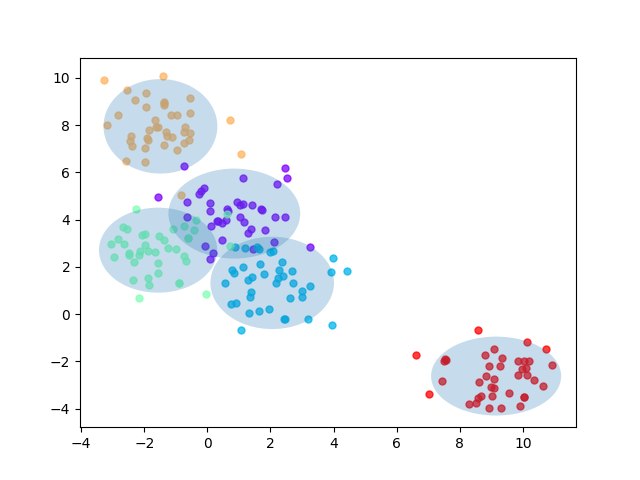
\includegraphics[scale = 0.75]{Figure_1.png}
    \caption{Guassian Confidence Intervals}
\end{figure}


\section*{Assignment 2}

In the function \texttt{computePrior} below we calculate the prior probabilities for each of the respective labels. 

\begin{lstlisting}
def computePrior(labels, W=None):
    Npts = labels.shape[0]
    if W is None:
        W = np.ones((Npts,1))/Npts
    else:
        assert(W.shape[0] == Npts)
    classes = np.unique(labels)
    Nclasses = np.size(classes)

    prior = np.zeros((Nclasses,1))
    
    for k in range(Nclasses):
        
        ind = np.where(labels == classes[k])[0]
        
        prior[k] = np.sum(W[ind])/np.sum(W)

    return prior
\end{lstlisting}

Using the previous function \texttt{mlParams} to compute the arrays $\boldsymbol\mu$ and $\boldsymbol\Sigma$ we can use \texttt{computePrior} to evaluate the posterior probabilities in the function \texttt{classifyBayes} which uses a naive bayes classifier to classify a set of points \texttt{X}.

\begin{lstlisting}
def classifyBayes(X, prior, mu, sigma):

    Npts = X.shape[0]
    Nclasses,Ndims = np.shape(mu)
    logProb = np.zeros((Nclasses, Npts))
    
    for k in range(Nclasses):
        
        diff = X-mu[k]
        
        logSigma = np.log(np.linalg.det(sigma[k]))/2
        
        logPrior = np.log(prior[k])
        
        for j in range(Npts):
            
            logProb[k][j] = -logSigma - np.inner(diff[j]/np.diag(sigma[k]), diff[j])/2 + logPrior

    h = np.argmax(logProb,axis=0)
    return h
\end{lstlisting}

\section*{Assignment 3}

We can use the aforementioned function \texttt{classifyBayes} to test how well it performs on separate data sets. The data sets that we have available are one containing data of different types of irises and one contains data for different vowels. 

We can plot the classification boundaries for the respective data sets as follows.

\begin{figure}
    \centering
    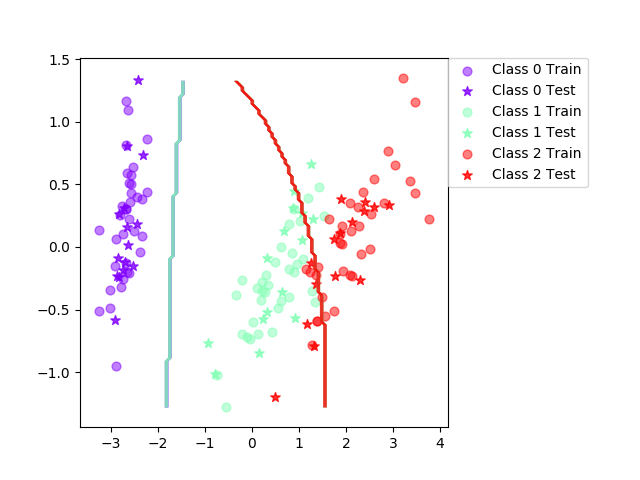
\includegraphics[scale = 0.75]{BayesIris.png}
    \caption{Bayes Classifier: Iries}
\end{figure}

\begin{figure}
    \centering
    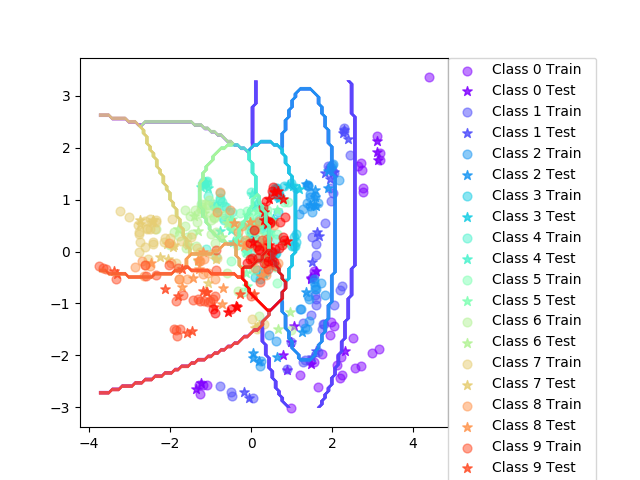
\includegraphics[scale = 0.75]{BayesVowel.png}
    \caption{Bayes Classifier: Iries}
\end{figure}

\section*{Assignment 4}






\end{document}
